%A compiler dans un terminal avec la commande "pdflatex -shell-escape Rapport_Pidash_Lentali.tex"
\documentclass{article}
\usepackage[utf8]{inputenc}
\usepackage{listings}
\usepackage{minted}
\usepackage[top=2cm, bottom=2cm, left=2cm, right=2cm]{geometry}
\usepackage{graphicx}


\title{Python \\Le Jeu de la Vie}
\author{Pidash Angelina\\ Lentali Thomas \\Université de Bordeaux }
\date{Décembre 2015}

%\lstset{escapechar=@,style=customc}
\begin{document}

\maketitle

\section{Introduction}
Ce projet a pour but de créer un programme sur le Jeu de la Vie de John Horton Conway en langage Python.\\
Nous allons travailler dans un environnement composé de:

\begin{itemize}
\item un temps discret,
\item un terrain de jeu - le plan, qui est constitué de cellules, chaque cellule a huit voisins,
\item de cellules qui peuvent avoir deux états distincts: mort ou vivant. La totalité des cellules vivantes est appelée génération.

\end{itemize}

\noindent Nous allons appliquer les règles classiques suivantes aux cellules:
\begin{itemize}
\item chaque génération est calculée à partir de la précédente,
\item une cellule devient vivante si elle a exactement 3 cellules vivantes comme voisins,
\item une cellule vivante continue à vivre, si elle a  2 ou 3 voisins vivants.
\end{itemize}

\section{Implémentation}

\subsection{Modèle de base}

Le fonctionnement de base du jeu de la vie est défini comme suit:
\begin{enumerate}
\item Créer un tableau à deux dimensions de valeurs booléennes, où "1" pour signifier la présence d'une cellule vivante, et "0" pour signifier l’état mort de la cellule,
\item Générer un nouveau tableau,
\item Pour chaque cellule, il faut déterminer le nombre de voisins vivant qui l'entoure et définir si une cellule commence à vivre pour la nouvelle génération ou non,
\item Le nouveau tableau est écrit à la place de l'ancien,
\item Revenir à l'étape 2.
\end{enumerate}

\noindent L'algorithme présente plusieurs inconvénients:
\begin{itemize}
\item  le temps d’exécution linéaire par rapport à la taille du champ.
\item La double consommation de mémoire (nécessaire pour stocker la génération précédente + nouvelle).
\item Il exige beaucoup de code à mettre en œuvre.
\end{itemize}

Ceci nous a poussé à repenser cette idée de réalisation et l'avons optimisé en éliminant les inconvénients cités précédemment.\\

\subsection{Amélioration du modèle}

Pour augmenter le confort d'utilisation de notre implémentation du Jeu de la vie, nous avons utilisé la bibliothèque graphique \textbf{\textit{Tkinter}}.

\begin{minted}{python}
from Tkinter import Tk, Canvas, Button, Frame, BOTH, NORMAL, HIDDEN
\end{minted}

\noindent On crée une fênetre:

\begin{minted}{python}
root = Tk()
\end{minted}

\noindent On définit la hauteur et la largeur de la fenêtre:

\begin{minted}{python}
win_width = 500
win_height = 500
config_string = "{0}x{1}".format(win_width, win_height + 32)
\end{minted}

\noindent A l'aide de la méthode \textbf{\textit{geometry()}}, nous définissons la taille notre fenêtre:

\begin{minted}{python}
root.geometry(config_string)
\end{minted}

\noindent Nous définissons la largeur d'une cellule:

\begin{minted}{python}
cell_size = 20
\end{minted}

\noindent On crée l'objet Canvas dans la fenêtre root dans lequel nous allons directement dessiner les cellules.

\begin{minted}{python}
canvas = Canvas(root, height=win_height)
canvas.pack(fill=BOTH)
\end{minted}

\noindent On détermine la taille du champ selon les cellules:

\begin{minted}{python}
field_height = win_height // a
field_width = win_width // a
\end{minted}

\noindent On crée le tableau unidimensionnel afin de garder les cellules.
\noindent On crée un Frame afin de garder les boutons:

\begin{minted}{python}
frame = Frame(root)
btn1 = Button(frame, text='Next generation', command = step) 
frame.pack(side='bottom')
\end{minted}

\noindent Ici nous permettons une relation entre mouvement de la souris (en cliquant) avec le Canvas grâce à la fonction \textbf{\textit{interpret}}:

\begin{minted}{python}
canvas.bind('', interpret)
root.mainloop()
\end{minted}

\subsection{Partie Fonctionnelle}

\noindent La fonction \textbf{\textit{interpret()}} récupère les coordonnées de la souris lorsque l'utilisateur clique une fois sur une case du Canvas ou, elle récupère une série de coordonnées lorsque l'utilisateur bouge sa souris sur le Canvas en maintenant le bouton gauche de la souris. Ces actions donne vie à une cellule morte.

\begin{minted}{python}
def interpret(e):   
    ii = (e.y-3) // cell_size
    jj = (e.x-3) // cell_size
    canvas.itemconfig(cell_matrix[addpoint(ii, jj)], state=NORMAL, tags='vis')
\end{minted}

\vspace{3mm}

\noindent La fonction \textbf{\textit{addpoint()}} convertit les deux dimensions de coordonnées dans l'adresse de notre un tableau en une dimension simple.

\begin{minted}{python}
def addpoint(ii,jj):
    if(ii < 0 or jj < 0 or ii >= field_height or jj >= field_width):
        return len(cell_matrix)-1  
    else:
        return ii * (win_width // cell_size) + jj
\end{minted}

\vspace{3mm}

\noindent Le rôle de la fonction \textbf{\textit{nextGeneration()}} est de:
\begin{itemize}
\item mettre à jour l'image,
\item calcul le nombre de voisins,
\item définit l'état d'une cellule en fonction du nombre de ses voisins .
\end{itemize}
Le statut de vie ou de mort de la cellule est géré avec des tags dans le canvas, "to vis" correspond à une cellule vivante, et "to hid" à une cellule morte:
\begin{minted}{python}
   if(vie[k]=="1"): 
      canvas.itemconfig(cell_matrix[addpoint(i, j)], tags=(current_tag, 'to_vis'))
   else:
      canvas.itemconfig(cell_matrix[addpoint(i, j)], tags=(current_tag, 'to_hid'))
\end{minted}

\vspace{3mm}

\noindent La fonction \textbf{\textit{repaint()}} a pour objectif de mettre à jour le Canvas avec les nouveaux états des cellules:
\begin{minted}{python}
def repaint():
  for i in range(field_height):
	for j in range(field_width):			
		if (canvas.gettags(cell_matrix[addpoint(i, j)])[1] == 'to_hid'):
			canvas.itemconfig(cell_matrix[addpoint(i, j)], state=HIDDEN, tags=('hid','0'))
		if (canvas.gettags(cell_matrix[addpoint(i, j)])[1] == 'to_vis'):
			canvas.itemconfig(cell_matrix[addpoint(i, j)], state=NORMAL, tags=('vis','0'))
\end{minted}

\vspace{3mm}

\noindent Lorsque l'on souhaite générer et afficher la nouvelle génération de cellules, nous appelons la fonction \textbf{\textit{step()}} qui elle même appelle les fonctions \textbf{\textit{nextGeneration()}} et \textbf{\textit{repaint()}}.

\newpage

\section{Intéraction Utilisateur-Programme}

Nous avons enrichi notre programme avec plusieurs options qui permettent à l'utilisateur d'agir sur le Jeu de la Vie (en plus d’être sensible aux clique de souris dans le Canvas).\\

\begin{figure}[H]
	\begin{center}
			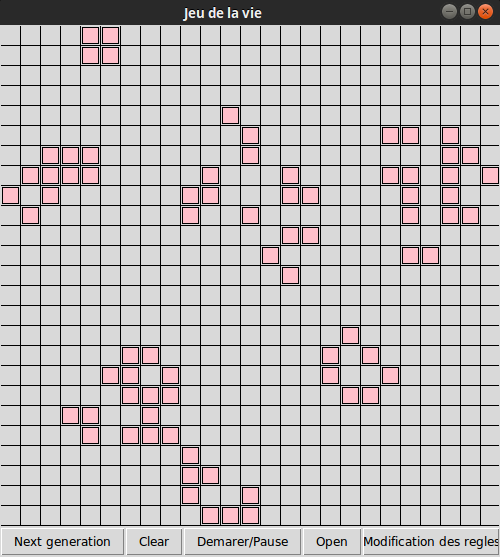
\includegraphics[scale=0.50]{capture_game.png}
         \end{center}
        \caption{Interface graphique du Jeu de la Vie}
	\label{desc}
\end{figure}

L'utilisateur peut notamment:
\begin{itemize}

\item afficher la nouvelle génération de cellules en appuyant sur le bouton \textbf{\textit{Next Generation}},

\item lancer de façon automatique les nouvelles générations en appuyant sur le bouton  \textbf{\textit{Automatique/Pause}} afin que l'utilisateur n'ai pas à cliquer sur \textbf{\textit{Next Generation}} pour générer une nouvelle génération à la fois,

\item appuyer sur ce même bouton \textbf{\textit{Automatique/Pause}} permet de mettre l’exécution automatique en pause, il suffit d’appuyer à nouveau sur ce même bouton pour relancer l’exécution automatique (principe "play/pause"),

\item effacer les cellules vivantes sur le canvas en cliquant sur \textbf{\textit{Clear}},

\item ouvrir une configuration du canvas enregistré sur un fichier au format .txt composé d'une matrice dont les "1" représentent les cellules vivantes et les "0" les cellules mortes, via le bouton \textbf{\textit{Open a File}}. En sélectionnant un fichier dans un dossier, on efface la configuration courante sur le canvas qui affiche la nouvelle configuration. Nous proposons un choix de configurations originales comme, par exemple, différentes tailles de vaisseaux:

\begin{minted}{python}

def file_to_open():
  file_path = askopenfilename()
  clear()
  try:
      ofi = open(file_path, 'rb')
  except:
      tkMessageBox.showwarning(
          "Open file", "Cannot open this file: (%s)\n" % file_path)
  compteur1 = 0
  for text in ofi:
      elt = text.split(' ')
      compteur2 = 0
      for x in range(len(elt)):
          if int(elt[int(x)]) == 1:
              canvas.itemconfig(cell_matrix[addpoint(compteur1,compteur2)],state=NORMAL,tags='vis')
          compteur2 += 1
      compteur1 += 1
\end{minted}

Exemple de fichier .txt lu par notre programme:
\begin{verbatim}
							0 0 0 0 0 0 0 0 0
							0 0 0 0 0 0 0 0 0
							0 0 0 0 0 1 0 0 0
							0 0 0 0 0 0 1 0 0
							1 0 0 0 0 0 1 0 0
							0 1 1 1 1 1 1 0 0
							0 0 0 0 0 0 0 0 0
							0 0 0 0 0 0 0 0 0
							0 0 0 0 0 0 0 0 0
\end{verbatim}

\item changer les règles de vie et de mort des cellules en cliquant sur le bouton \textbf{\textit{Modification des règles}}. En cliquant, une petite fenêtre s'ouvre et demande à l'utilisateur d'entrer les nouvelles règles au format binaire. Une fois les règles sont tapé dans la entry box, l'utilisateur doit cliquer sur le bouton \textbf{\textit{Changer les règles}}. Un second bouton, appellé \textbf{\textit{Règles de base}} permet de réinitialiser les règles originale du jeu et un troisième bouton,  ferme la fenêtre. Les erreurs sont gérées au niveau de la saisie de la nouvelle règle.

\begin{minted}{python}
def new_rules():
  global  e1, e2, new_vie, new_mort
  ask_rules = Tkinter.Toplevel(root)
  ask_rules.title('New Rules')
  ask_rules.geometry('450x80')
 
  l1 = Tkinter.Label(ask_rules).grid(row=0,column=0)
  e1 = Tkinter.Entry(ask_rules)
  e1.grid(row = 0, column = 1)
 
  l2 = Tkinter.Label(ask_rules).grid(row=1,column=0)
  e2 = Tkinter.Entry(ask_rules)
  e2.grid(row = 1, column = 1)
 
  Button(ask_rules,command=ask_rules.destroy).grid(row=2, column= 1)
  Button(ask_rules,command=default_values).grid(row=2, column= 2)
  Button(ask_rules,command=change_values).grid(row=2, column= 0)
 
  root.mainloop()
\end{minted}

\end{itemize}

\section*{Conclusion}

Ce projet nous a permis de pousser plus loin nos compétences en programmation.\\
Que ce soit du point de vu algorithmique avec l’amélioration de la structure de base du jeu de la vie et aussi du point de vu technique en créant une interface graphique qui peut notamment interagir directement avec les mouvements de la souris de l'utilisateur ainsi que la création de multiples fonctions utilisant différentes bibliothèques.





\end{document}

